%%%%%%%%%%%%%%%%%%%%%%%%%%%%%%%%%%%%%%%%%%%%%%%%%%%%%%%%%%%%%%%%%%%%%%%%
% Plantilla TFG/TFM
% Universidad de A Coruña. Facultad de Informática
% Realizado por: Welton Vieira dos Santos
% Modificado: Welton Vieira dos Santos
% Contacto: welton.dossantos@udc.es
%%%%%%%%%%%%%%%%%%%%%%%%%%%%%%%%%%%%%%%%%%%%%%%%%%%%%%%%%%%%%%%%%%%%%%%%


\chapter{Modelo de conocimiento}
\newpage
\section{Fase de identificación}
\subsection{Tareas del formulario OM-3}
La tarea elegida para este modelo conceptual ha sido la tarea 5 del OM-3 (Tabla \ref{tab:IdentificacionOM3}), que corresponde con la \textbf{Gestión de las Operativas Abiertas}.

\begin{table}[H]
  \centering
  \resizebox{18,0cm}{!}{
    \begin{tabular}{|c|c|c|c|c|c|c|}
      \hline
      \multicolumn{3}{|c}{\textbf{Modelo de Organización}} & \multicolumn{4}{|c|}{\textbf{Formulario OM-3: Descomposición de los Procesos}}\\
      \hline \hline
      \textsc{N\textordmasculine} & \textsc{Tarea} & \textsc{Realiza\-da por} & \textsc{¿Dónde?} & \textsc{Recursos de Conocimiento} & \textsc {¿In\-ten\-si\-va en Conocimiento?} & \textsc{Im\-por\-tan\-cia} \\
      \hline
            
      5 & \multicolumn{1}{|p{6.0cm}|}{\centering Gestionar las operativas abiertas} & \multicolumn{1}{|p{6.0cm}|}{\centering Inversor (usuario)} &  \multicolumn{1}{|p{5.0cm}|}{\centering En PC del inversor (usuario)} & \multicolumn{1}{|p{6.0cm}|}{\centering Experiencia en gestionar las operativas de compra y venta de activos al mercado de divisas. Teorías de gestión de capital de inversión} & Sí (elevado) & Máxima \\
      \hline
    \end{tabular}
  }
	\caption{\label{tab:IdentificacionOM3}Tarea elegida para el modelo de conocimiento}
\end{table}

\subsection{Glosario de términos}
\begin{itemize}
	\item \textbf{Activo:} Entidad en la que se prentende especular, que en caso de Forex, hay una variabilidad de 26 pares de divisas, por ejemplo, EURUSD - Euro contra el Dolar.
	\item \textbf{Tendencia Alcista:} es una tendencia del mercado bulsátil donde los precios de los activos financieros llegan a nuevos máximos comparando en un mismo período de análisis. Ejemplo en la imagen de la izquierda de la Figura \ref{fig:EjemploTentendias}.
	\item \textbf{Tendencia Bajista:} es una tendencia del mercado bulsátil donde los precios de los activos financieros llegan a nuevos mínimos comparando en un mismo período de análisis. Ejemplo en la imagen de la derecha de la Figura \ref{fig:EjemploTentendias}.
\end{itemize}

\begin{figure}[H]
	\centering
	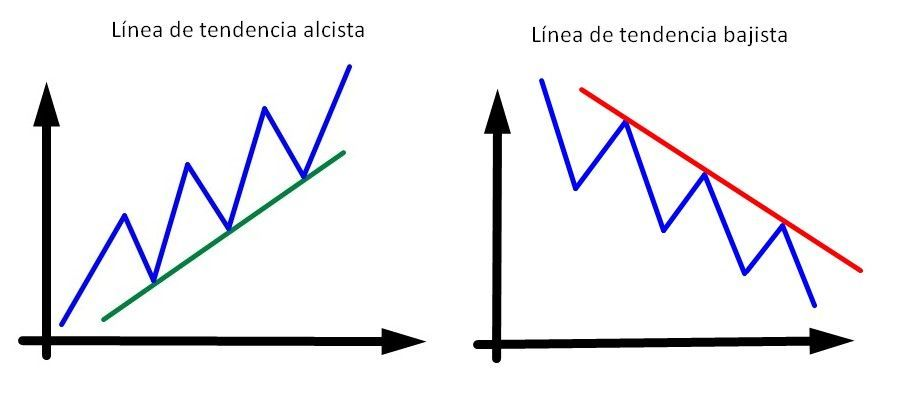
\includegraphics[scale=0.50]{imagenes/EjemploTentendias.png}
	\caption{\label{fig:EjemploTentendias}Ejemplo de tendencias de mercado}
\end{figure}

\subsection{Descripción de escenarios}
\begin{enumerate}
	\item primer escenario 
	\item segundo escenario 
\end{enumerate}

\section{Fase de especificación}
\subsection{Justificación de la selección de la metodología}

\subsection{Plantilla anotada}
